\section{Nuclear physics}

\subsection{Nuclear shell model} \label{sec:nuclear model}
The atom is build up of electrons around a nucleus of protons and neutrons.
The electric coulomb forces keep the negatively charged electrons around the positively charged
protons in the nucleus. The protons and the neutrons are bound together by the strong nuclear force.
See figure \ref{img:atomic-structure} for illustration.

The quantum mechanical model of the atom is build up by quantum particles (electrons)
in the coulomb potential of the nucleus. The energy of the electrons is defined by their
radial quantum number, angular momentum quantum number, and intrinsic spin (analogous to
rotation about the particles own axis).

The strong force that holds the core together is not as well understood as the electric coulomb
force. In order to make a quantum mechanical model of the core it is assumed that all the
particles in the nucleus combined make up a central, harmonic potential. The protons and neutrons are
then modelled as quantum mechanical particles in the central field.
The states of the different particles is given by the principle quantum number $n$,
the orbital angular momentum quantum number $l$, and the total angular momentum quantum number $j=l\pm\frac{1}{2}$.
Similar to the aotmic model\mycitetwo{basdevant2005}{ch.2.4}.
The energy of these state do not stack linearly, but group together in a seemingly clumsy manners.
If particularly many energy states are grouped together, and the binding energy of nucleons peaks,
the group is called a magic number (see figure \ref{img:nuclear-shells}).

%Nuclear mass, binding energy, and reactions
\subsection{Mass and binding energy} \label{sec:binding-energy}
The total mass of the nucleus is given by the sum it's consituents, the nucleons.
Dividing by the mass number (number of nucleons in the core) one gets the average mass per nucleon.
This should be pretty elementary, but it turns out that the mass per nucleon dimishes
as mass number increases. Each proton and neutron becomes lighter as more protons and neutrons are stacked
into the central potential of the nucleus.
This energy is analogous to the energy needed to release nucleons from the nucleus potential\mycite{iliadis2015}.
See figure \ref{img:binding-energy-curve} to see how the average binding energy per nucleon evolves with number of nucleons in the nucleus.
\noindent
A classical example is two lighter nuclei colliding to one heavier nucleus. Since
the mass per nucleon is lower, but the total number of particles before and after has not changed the total
energy has lowered. This excess energy (or mass) is radiated away as thermal photons.
This implies that synthesizing heavier elements up to iron (peak binding energy in figure \ref{img:binding-energy-curve}) from
lighter elements releases energy.
Since protons and neutrons are fermions they follow the Pauli exclusion principle,
stating that a maximum of two particles can exist in any given quantum state in a bound system, and they must have opposite spins to do so\mycitetwo{basdevant2005}{ch.1.7.3}.
\noindent
E.g. Take a nucleus and continue to stack neutrons onto it, as the neutrons take on
higher and higher energy states (from the Pauli exclusion principle) the nucleus eventually reaches
a level where any new neutron would no longer be bound. The neutrons would therefore be immediately expelled.
If some protons were added, the strong force would be even stronger and more neutrons could be
added to the nucleus. The reverse is also true if protons were added continously.
This point in the nuclear chart (neutron number - proton number map) is called the neutron drip line
and proton drip line respectively\mycite{iliadis2015}.

\subsection{Reaction rates} \label{sec:reaction-rates}
A nuclear reaction in stellar environments is usually depicted as two quantum particles, 1 and 2,
interacting to make two new quantum particles, 3 and 4.
\noindent
Written as: $1+2 \rightarrow 3+4$ or $1(2,3)4$ where 2 and 3 are \textit{usually} the lighter particles
``impacting onto'' or ``emitting from'' the larger nuclei 1 and 4.
If particle 2 is a photon, (absorption of light), the process is a photodisintegration process and the
energy released is negative.
If particle 3 is a photon, then energy is created from two nuclei colliding and merging to a single nucleus,
the energy released is positive.
The probability of a given reaction happening is called the nuclear cross-section, and is measured per area.
The cross-section is velocity dependant, so the reaction probability in a stellar volume is therefore the integral of cross-section over the velocity distribution. For thermal velocities in an ideal gas the Maxwell distribution\mycite{maxwell60} can, and is usually adopted\mycite{iliadis2015}.
The reaction rate then is the probability times the number density of each nuclear specie, as more particles closer together means
more possible reactions\mycite{iliadis2015}.
The end result is that nuclear reactions are dependent on the density and
thermal velocity (temperature) in stellar environments, and produces energy as long as
the fusing particles are lighter than iron.

%weak interactions
\subsection{Weak interactions and \betadecay} \label{sec:betadecay}
Interactions with the weak force cause different decay reactions. The most common weak interactions are listed below
\begin{description}
  \item[free neutron decay] \ce{n \rightarrow p^+ + e^- + $\bar{\nu_e}$} \\
  \item[\betadecay] \ce{^{A}_{Z}X_{N} \rightarrow ^{A}_{Z+1}Y_{N-1} + e^{-} + $\bar{\nu_e}$} \\
  \item[$\beta^+$ decay] \ce{^{A}_{Z}X_{N} \rightarrow ^{A}_{Z-1}Y_{N+1} + e^{+} + \nu} \\
  \item[electron capture] \ce{^{A}_{Z}X_{N}  + e^{-} \rightarrow ^{A}_{Z-1}Y_{N+1} + \nu} \\
  \item[anti-neutrino capture] \ce{^{A}_{Z}X_{N} + $\bar{\nu}$ \rightarrow ^{A}_{Z+1}Y_{N-1} + e^{-}} \\
  \item[neutrino capture] \ce{^{A}_{Z}X_{N} + \nu \rightarrow ^{A}_{Z-1}Y_{N+1} + e^{+}} \\
\end{description}

%beta decay probability
The \betadecay transitions depend on the initial and final quantum states of the entire nucleus.
Transitions which are independant lepton energies are most likely to occur (out of all the weak interactions considered)
and are called allowed transitions.
The forbidden transitions are weak interactions that are less probable.
%beta decay in stellar plasma
In stellar environments, with high temperatures the nuclei in question can be excited to higher energies.
The increased number of possible states increases the net reaction probability and therefore the overall decay rate.
This also means that the chance of observing forbidden transitions is higher.
%radioactive decay
Assuming that a radioactive decay occurs at a random point in time, with a uniform distribution in time,
The probability of decay of a single particle is proportionale with time.
The probaiblity of decay of two particles will be twice as much, meaning decay probability is
proportional to the amount of radioactive particles present.
Consider then an amount of particles, N,  large enough to turn probability into observable decays,
even at infinitesimal timescales. The number of decays, d$N$, is then given by:
\begin{equation}
  \begin{array}{rl}
    \textrm{d}N &\propto N \textrm{d}t \\
    \textrm{d}N &= C_{\textrm{decay}} N \textrm{d}t = -\lambda N \textrm{d}t\\
    \frac{\textrm{d}N}{\textrm{d}t} &= -\lambda N \\
    N(t) &= N_0 e^{-\lambda (t - t_0)}
  \end{array}
  \label{eq:decay-diff-eq}
\end{equation}
d$t$ is the infinitesimal timeinterval.
$C_{\textrm{decay}}$ is the proportionality constant.
Since the decay-process removes number of atoms from the nuclear specie, it will always be negative.
$\lambda$ is the positive proporitonality constant, called the decay constant (because it will not change for a given reaction with constant density and constant temperature).

Solving the differentialequation, eq.\ref{eq:decay-diff-eq}
gives the time evolution of numbers of particles, given and initial abundance $N_0$ at time $t_0$.
The half-life is the time when the abundance is half it's orginial value, $T_{1/2} = \frac{\ln 2}{\lambda}$, while
mean lifetime is the average lifetime integrated for all particles $\tau = \lambda^{-1}$.\\
%half-life of free neutrons, C-14, Re-187
Some relevant half-lifes free neutrons, \isotope{14}{6}{C}, \re{187}.
\newcommand\myfootnotenumber{1}
\footnotetext[\myfootnotenumber]{\href{https://www-nds.iaea.org/relnsd/vcharthtml/VChartHTML.html}{IAEA Nuclear Data Service Livechart}}
\newcommand\appspace{\textrm{\vspace{1cm}}}
\begin{align*}
  T_{1/2}(n) &= 10.2 \textrm{ min} &\appspace \textrm{from \mycitetwo{iliadis2015}{ch.1.8}} \\
  T_{1/2}(\isotope{14}{6}{C}) &= 5700 \textrm{ yr} &\appspace \textrm{from NDS\footnotemark[\myfootnotenumber]} \\
  T_{1/2}(\textrm{\re{187} ground state}) &= 4.33 \times 10^{10} \textrm{ yr} &\appspace \textrm{from NDS\footnotemark[\myfootnotenumber]} \\
  T_{1/2}(\textrm{\re{187} first excited state}) &= 4.33 \times 555.3 \textrm{ ns} &\appspace \textrm{from NDS\footnotemark[\myfootnotenumber]} \\
  T_{1/2}(\textrm{\re{187} second excited state}) &= 4.33 \times 114 \textrm{ ns} &\appspace \textrm{from NDS\footnotemark[\myfootnotenumber]} \\
\end{align*}
Chart of nuclides is a two dimensional map of all nuclides with amount of protons on the y-axis and neutrons on the x-axis. A small section of the isotopes between \isotope{H}{1}{1} and \isotope{Fe}{26}{52} can be found in figure \ref{img:nuclide-chart-lowmass}.
\begin{figure}
  \centering
\includegraphics[width=\figwidth]{img/nds_nuclide_chart.png}
\caption[Chart of Nuclides: low-mass excerpt]{
\label{img:nuclide-chart-lowmass}
Excerpt from low-mass region of the chart of nuclides. \\
Relevant colors: {Black - stable isotopes}, {cyan - \betadecay unstability}, {green - $\beta^+$-decay unstability}, {orange - proton emission}, {magenta - neutron emission}. \\
Image credit: IAEA Nuclear Data Services Livechart; \href{https://www-nds.iaea.org/relnsd/vcharthtml/VChartHTML.html}{NDS livechart}, retrieved 24.05.18.
}

\end{figure}

%thermonuclear reactions
%q-value and cross-sections
%rate of nuclear reactions
%abundance evolution

%nuclear burning
%hydrostatic hydrogen burning
%hydrostatic helium burning
%carbon burning
%neon burning
%oxygen burning
%silicon burning
%explosive burning in CCSN

%nucleosynthesis beyond iron peak
\subsection{Nucleosynthesis beyond iron}
For elements heavier than iron, collision with other elements will cost energy instead of release energy.
In stellar environments, the temperatures and excess energies are very high so some heavier elements can form from
energetic light particles colliding with energetic iron particles. However this will be in trace amounts
and does not explain the relatively high amount of heavy elements found in the solar system\mycite{iliadis2015}.

In order to create heavier elements than iron, seeds close to the iron peak (see figure \ref{img:binding-energy-curve})
are bombarded by lighter particles, like neutrons and protons, in order to increase mass-number one collision at a time.
These processes of creating heavier elements are called proton capture process and neutron capture processes.
Due to the additional coulomb barrier between protons, neutron capture processes are more probable and likely to occur\mycite{iliadis2015}

\subsubsection{Slow neutron capture process} \label{sec:sncp}
Imagine a stream of neutrons onto some heavy seed nuclei, Two competing reactions take place.
The capture of a neutron onto the seed nuclei and the radioactive $\beta^-$-decay
(in a neutron-heavy nucleus the electron emission is more probable then the positron emission).

%s-process
If the neutron capture is much slower then the radioactive decay, any new
isotope must be stable or will decay to a stable isobar with the same mass number. This is called the slow neutron capture process, or s-process for short.
It will create heavy nuclei along the valley of stability\footnote{line of stable nuclei in the chart of nuclides, see black colored squares in figure \ref{img:nuclide-chart-lowmass}}.
For such a process to occur in stellar environments there must be access to a high density of neutrons and heavy seed nuclei from the iron peak.
The heavy seed nuclei can just as easily have been produced by another massive star and ejected into the interstellar medium. Free neutrons on the other hand have a short lifespan and must have been created in the local environments.
Some processes in the hydrostatic helium burning processes produce excess amounts of neutrons, as do the subsequent $\alpha$-capture processes in carbon burning.
In addition to high neutron density requirements, the temperature must be high enough for thermal reactions to occur, but can not be so hot that most of the heavy seed nuclei are photodisintegrated before a significant amount of heavy nuclei can be synthesized.
This means that the optimal site for most of s-process nucleosynthesis is the late time helium-burning phase of stars with relatively low mass. These are asymptotic giant branch stars with mass below roughly three solar masses\mycite{iliadis2015}.
Numerical nuclear reaction networks in stars of this kind have lead to synthesis distributions that correspond with s-only abundances in the solar system.
The exact site can include many stellar mass range and mixing episodes between different layers of the stellar interior, which can cause some new sites.
\comment{\\ Abundances by Suess and Urey, (s+r)-processes suggested by BBFH, review by iliadis- and basdevant-books}
\comment{\\ Classic stellar model paper, Arnould?}
\comment{\\ sncp-images}
\comment{hereby named the s-process}

\subsubsection{Rapid neutron capture process} \label{sec:rncp}
%r-process
Modelling the s-process contributions and scaling them to fit the solar observed number abundances results in a differential pattern with clear structure.
There are uncertainties in the s-process contribution, and solar observed abundances as well, but some nuclei cannot be produced by regular slow neutron capture process.
A rapid neutron capture process is required, and such a process adds to many nuclei already ``filled partially'' by the s-process to account for the observed solar abundances\mycite{arnould07}.
This pattern is from a separate process called rapid neutron capture process, where the neutron capture rate is much higher than the $\beta^-$-decay rate. In such a process the heavy seed nuclei (assumed to be iron peak nuclei from a old supernova), will capture many neutrons until the nucleus is saturated with neutrons.
At that point neutrons are emitted away as soon as they are captured.
A distribution of neutron-heavy isotopes for a given seed specie is then left over time, kept in equilibrium by the constant bombardment of high energy neutrons.
The distribution will have a maximum given by the equilibrium conditions where most heavy isotopes will reside.
The nuclei in greatest abundance will \betadecay (to an isobar with greater atomic number) in greatest abundance.
In the heavier elements the process begins anew, with neutrons captured onto the nucleus and eventually escaping until an equilibrium distribution is reached. This process is faster than the $\beta^-$-decay process (by definition) and will reach equilibrium before a significant fraction of nuclei decay to isobars with higher atomic number.
When the high energy neutrons are no longer available in the same quantities, the r-process will stop and leave distributions of neutron-heavy isotopes that eventually will decay to stable isotopes far heavier than iron\mycite{iliadis2015}.
This sort of process require a much higher number density of neutrons than the s-process described above, and the scales of $10^{21} cm^{-3}$.
The astrophysical site, and details, of this process, are greatly debated.
\comment{reference to debate of r-process sites}
The output yields of the process are observed in our sun as well as old stars, but these stars could not have created those elements themselves so the process must be relatively quick in order to eject elements into the interstellar medium to be absorbed by our sun and other older stars.
\comment{hereby named the r-process}

\subsubsection{Proton capture process}
%briefly mention p-process
The same capture process can happen to the proton heavy side of nuclei, with dense regions of high energy protons. This is less likely to occur due to the added repulsive coulomb force and will therefore have smaller rates, but is necessary to explain the natural occurance of some isotopes in the nuclear chart\mycite{iliadis2015}.

\subsubsection{Distributions of neutron capture processes} \label{sec:nuclear-processes-distributions}
\comment{\\ include image of isotope equilibrium distributions here}
\comment{\\ include r-process pattern here}
\comment{\\ include plot about s-process r-process in nuclear chart}
\comment{\\ see path:} \verb|/other_data/arnould_plots/etc|

\begin{figure}
  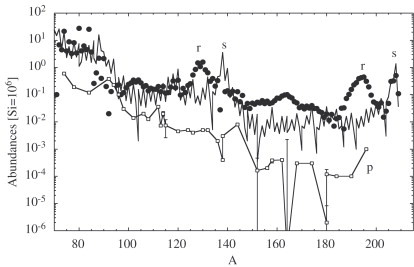
\includegraphics[width=0.5\textwidth]{other_data/arnould_plots/fig1_p100_arnould07_process_decomp.jpg}
  \includegraphics[width=0.5\textwidth]{other_data/arnould_plots/fig4_p220_landholt93_sncp.png}
  \includegraphics[width=0.5\textwidth]{other_data/arnould_plots/fig5_p209_landholt93_rncp.png}
  \includegraphics[width=0.5\textwidth]{other_data/arnould_plots/fig7_p211_landolt93_sos.png}
\end{figure}

In this project, the r-process is of most interest, since the abundance of \re{187} is solely determined by r-process events and the s-process sites are less debated.
\comment{\\discuss possible sites}

\subsection{Stellar enhancement factor} \label{sec:sef}
The \betadecay of a given nuclei in a given energy state is determined by it's halflife (or decay-constant).
This means that a nuclide heated to an excited energy state can have a vastly different halflife than  it's ground state.
This is true for re{187}, among other radioactive nuclei.
These excited stages have greatly reduced lifespans (see section \ref{sec:betadecay} for more details).
In neutral gas in the interstellar medium the temperatures and densitites are not high enough to excited nuclear states, but stellar environments is another story.
If significant populations of \re{187} reach excited nuclear states, halflife of \re{187} will significantly reduce (meaning the decay-constant will increase).
In order to estimate how such environments affect the decay-constant, an \textit{stellar enhancement factor}, SEF, is considered\mycite{shizuma05}. Where $\lambda_{\scriptscriptstyle \beta}^{\scriptscriptstyle \textrm{eff}} = \textrm{SEF}\times\lambda_{\scriptscriptstyle \beta}$ is the effective \betadecay-constant and $\lambda_{\scriptscriptstyle \beta}$ is the \betadecay-constant for the ground state.
In \mycite{shizuma05} a stellar enhancement factor of $\textrm{SEF}=1.2$ is adopted.

\subsection{Nuclear figures}

\begin{figure}
  \begin{minipage}{0.49\textwidth}
    %use \paperheight as fig-height
%\begin{figure}
  \centering
  \includegraphics[width=\linewidth]{img/nuclear_shells.png}
  \caption[Nuclear shells]{
    \label{img:nuclear-shells}
    Energy states of the nuclear orbitals/shells. This shows how the energy-states group together to form clusters of energy-states separeted by so-called magic numbers.\\
    The energy states are grouped together by their principle quantum number $n$, with their orbital splitting $l$ shown in the left column. As can be seen, each orbital term greater then zero (s=0, p=1, ...) are split into two sub-levels determined by their spin-orbit terms in the second column from the left. The third column represent the number of nucleons possible per level, and the far right column indicate magic numbers\mycite{basdevant2005}{ch.2.4}.\\
    Image credit: Bakken at English Wikipedia [CC BY-SA 3.0], from Wikimedia Commons
  }
%\end{figure}

  \end{minipage}
  \begin{minipage}{0.49\textwidth}
    %Draw atomic structure with nucleus and electrons in simple Bohr-model form
\newlength\elrad
\newlength\prorad
\newlength\orbit
\setlength\elrad{0.5mm}
\setlength\prorad{2\elrad}
\setlength\orbit{1cm}

\newcommand\particle[4]{\draw[fill=#4] (#1,#2) circle [radius=#3]}
\newcommand\electron[2]{\particle{#1}{#2}{\elrad}{blue}}
\newcommand\neutron[2]{\particle{#1}{#2}{\prorad}{gray}}
\newcommand\proton[2]{\particle{#1}{#2}{\prorad}{red}}

\centering
\begin{tikzpicture}
    %nucleus
    \proton{-\prorad}{0};
    \proton{\prorad}{2\prorad};
    \proton{\prorad}{-2\prorad};
    \proton{-2\prorad}{\prorad};
    \proton{-2\prorad}{-\prorad};
    \proton{3\prorad}{0};
    \neutron{\prorad}{0};
    \neutron{-\prorad}{2\prorad};
    \neutron{-\prorad}{-2\prorad};
    \neutron{2\prorad}{\prorad};
    \neutron{2\prorad}{-\prorad};
    \neutron{-3\prorad}{0};
    %inner orbit
    \draw (0,0) circle [radius=\orbit];
    \electron{0}{\orbit};
    \electron{0}{-\orbit};
    %outer orbit
    \setlength\orbit{2\orbit}
    \draw (0,0) circle [radius=\orbit];
    \electron{0}{\orbit};
    \electron{0}{-\orbit};
    \electron{\orbit}{0};
    \electron{-\orbit}{0};
\end{tikzpicture}
\caption[Atomic structure]{\label{tikz:atomic-structure}
    Figurative representation of a \isotope{C}{6}{12}-atom with six protons, neutrons, and electrons. The protons (red) and neutrons (gray) occupy the nucleus in the center, while the electrons (blue) orbit around them. According to quantum physics the electrons do not rotate around the nucleus in spherical orbits, but occupy orbitals/energy states around the nucleus as probability distributions. Real and relative sizes do not apply.
    }
  

    %\begin{figure} 
\centering 
\includegraphics[width=\linewidth]{img/binding_energy_curve.png}
\caption[Binding energy per nucleon]{\label{img:binding-energy-curve}
The binding energy per nucleon in the nucleus for isotopes up to \isotope{U}{92}{238}. The peak at \isotope{Fe}{26}{56} means that the nucleons are most tightly bound, and have the least amount of potential energy. \\
Image Credit: Wikipedia Commons
}
%\end{figure}

  \end{minipage}
\end{figure}

\FloatBarrier
